\documentclass[a4paper,10pt]{article}

\usepackage{tikz}
\usepackage{fullpage}
\usepackage{amsmath,amsthm,amsfonts,amssymb,amscd}
\usepackage{mathtools}
\usepackage{colortbl}
\usepackage{xcolor}
\usepackage{graphicx}
\usepackage{titlesec}
\usepackage{xepersian}
\usepackage{multirow}

% ---------------------------
%      Dark Theme Setup
% ---------------------------
\definecolor{CustomBackground}{HTML}{1C1C1C}  % Dark background
\pagecolor{CustomBackground}
\color{white}

% ---------------------------
%        Font Setup
% ---------------------------
\settextfont{Vazir.ttf}[
    BoldFont = Vazir-Bold.ttf,
    Path = fonts/
]
\setlatintextfont{Vazir.ttf}[
    BoldFont = Vazir-Bold.ttf,
    Path = fonts/
]

% ---------------------------
%     Custom Adjustments
% ---------------------------
\renewcommand{\baselinestretch}{1.2}
\renewcommand{\thesection}{\arabic{section}}
% User-defined commands for homework info (adjust as needed)
\newcommand{\HomeworkNumber}{5}
\newcommand{\HomeworkDeadline}{1404/09/01}
\newcommand{\id}{\texttt{\detokenize{@HESAMODIN83}}}




\begin{document}

% ---------------------------------
%           Front Page
% ---------------------------------
\begin{titlepage}
    \begin{center}
        \vspace*{1cm}
        % Bigger Logo
\begin{figure}
    \centering
    
\includegraphics[width=0.3\linewidth]{assets/fum-logo.png}
    \label{fig:placeholder}
\end{figure}
        {\Huge \bfseries مبانی و کاربردهای هوش مصنوعی}\\[0.5cm]
        {\Large دانشگاه فردوسی مشهد}\\[0.3cm]
        {\Large گروه مهندسی کامپیوتر}\\[0.5cm]
        {\normalsize دکتر هراتی}\\[2cm]

        {\Huge \bfseries تمرین \HomeworkNumber}\\[0.5cm]
        {\Large مهلت تحویل: \HomeworkDeadline}\\[2.5cm]

        \Large مسئول تمرین: \id
    \end{center}
\end{titlepage}

% ---------------------------------
%          Instructions
% ---------------------------------
\clearpage
\section*{دستورالعمل‌ها}

دانشجویان محترم لطفا به موارد زیر توجه فرمایید:
\begin{itemize}
\itemsep0em
\item
	تحويل تمرين‌ها فقط از طريق سامانه  آموزش مجازی دانشگاه امکان‌‌پذیر است.
\item 
	تمرین‌ها باید دست نویس، خوانا و با استفاده از خودکار آبی یا مشکی و یا به صورت دیجیتالی با استفاده از قلم نوری نوشته شوند. 
\item
از تمرین های حل شده دیگران و هوش مصنوعی استفاده نکنید. پیامد های این کار با دانشجو می باشد.
\item
	نوشتن جواب آخر به تنهايى نمره‌ای نداشته و تمام مراحل حل، مشمول نمره می‌باشد.
\item 
	به دلیل موعد از پیش تعیین شده تمرین‌ها و برنامه درسی، امکان تمدید تمرین وجود ندارد. همچنین بدیهی است که ارسال تمرین پس از موعد تعیین شده نمره‌ای نخواهد داشت.
	
\item نحوه نام‌گذاری فایل پاسخ باید مطابق جدول ~\ref{tab:file_format}
و به شکل pdf باشد.

\begin{table}[h]
	\centering
	\begin{tabular}{|c|c|}
		\hline
		\textbf{Format} & \texttt{StudentID-Full\_Name-\#HwNo.pdf} \\
		\hline
		\textbf{Example} & \texttt{9876543210-Alan\_Turing-\#05.pdf} \\
		\hline
	\end{tabular}
	\caption{شیوه نام‌گذاری فایل‌ها}
	\label{tab:file_format}
\end{table}
    
    
\end{itemize}
\rule{\linewidth}{0.4pt}


%  هر سوال که گذاشته میشه، حما 3 خط آخر رو هم بعد از اتمام نوشتن سوال بگذارید.
% \bigskip
% \bigskip
% \hline


\section{سوال اول}

صحیح و غلط بودن جملات زیر را مشخص کنید و توضیح کوتاه دهید.

\begin{enumerate}
    \item الگوریتم‌های Arc-Consistency مانند AC-3 باعث می‌شوند که در مسائل CSP دیگر نیازی به Backtracking وجود نداشته باشد.\\

    \item برخلاف AC-3، روش Checking Forward ممکن است ناسازگاری‌های غیرمستقیم  را تشخیص ندهد.\\

    \item استفاده از MRV باعث افزایش احتمال حرکت به سمت بن‌بست‌های دیرهنگام می‌شود.\\
    
    \item استفاده از Arc-Consistency سرعت جستجو را همیشه افزایش می‌دهد.\\

\end{enumerate}

\bigskip
\bigskip
\rule{\linewidth}{0.4pt}

\section{سوال دوم}

توضیح دهید چرا در انتخاب متغیرها، متغیری که بیشترین محدودیت را دارد  ولی در انتخاب مقادیر، مقداری که کمترین محدودیت را ایجاد می‌کند  در جستجوی CSP یک هیورستیک خوب محسوب می‌شود؟


\bigskip
\bigskip
\rule{\linewidth}{0.4pt}

\section{سوال سوم}

با توجه به اینکه CSP ها با \lr{preferences} را می‌توان با روش‌های جستجوی بهینه‌سازی حل کرد:

\begin{enumerate}
    \item[الف.] توضیح دهید \lr{Constraint Optimization Problem (COP)} چیست و چه تفاوتی با \lr{CSP}های معمولی دارد.
    \item[ب.] بیان کنید چرا اضافه شدن \lr{preferences} به \lr{CSP} باعث می‌شود که استفاده از روش‌های جستجوی بهینه‌سازی مناسب‌تر باشد.
    \item[ج.] یک مثال از مسائل قابل حل با \lr{COP} را ذکر کنید.
\end{enumerate}


\bigskip
\bigskip
\rule{\linewidth}{0.4pt}

\section{سوال چهارم}


در یک جدول متقاطع (\lr{crossword puzzles})، متشکل از خانه‌های مسدود و غیرمسدود است که همچنین یک لیست از لغات نیز دارد. هدف ما این است که به هر خانه غیرمسدود یک حرف اختصاص دهیم به گونه‌ای که هر قطعه‌ی پیوسته از خانه‌های غیرمسدود که به صورت افقی یا عمودی کنار هم قرار گرفته‌اند، یک کلمه‌ی معتبر از فرهنگ لغت را تشکیل دهد.
مثالی از یک جدول کلمات متقاطع حل شده در ادامه آمده است:

\begin{center}
    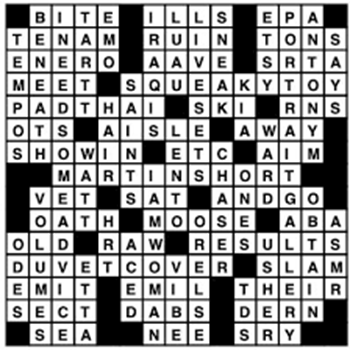
\includegraphics[width=0.3\textwidth]{assets/crossword-puzzle.png} % مسیر عکس را تغییر دهید
\end{center}
این مسئله را به عنوان یک مسئله‌ی ارضای محدودیت به دو شکل متفاوت فرموله و مدلسازی کنید. در هر دو فرموله، متغیرها، دامنه‌ها و محدودیت‌ها به شکل کامل و دقیق مشخص کنید.


\bigskip
\bigskip
\rule{\linewidth}{0.4pt}


\section{سوال پنجم}
برنامه روز شنبه کلاس‌های یک دانشکده، شامل ۷ گروه درسی است و این ۷ گروه باید در یکی از سه کلاس دانشکده (\lr{R1,R2,R3}) تشکیل شوند. بدیهی است هیچ دو گروه درسی، همزمان در یک کلاس تشکیل نخواهند شد.
\begin{center}
    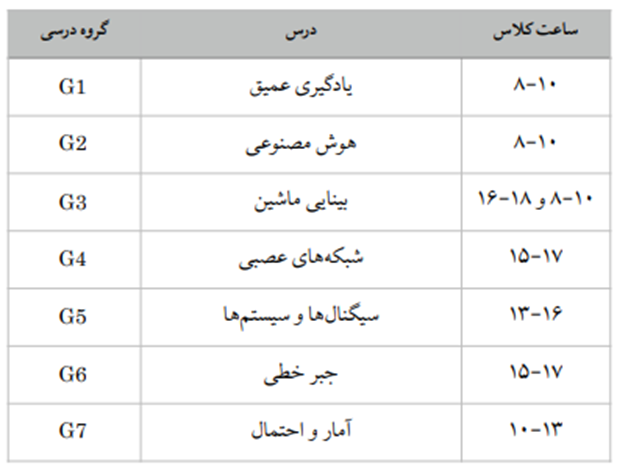
\includegraphics[width=0.5\textwidth]{assets/image.png} % مسیر عکس را تغییر دهید
\end{center}
\textbf{محدودیت‌ها}

\begin{itemize}
    \item کلاس \(R3\) به دلیل کوچک بودن، برای گروه‌های \(G7\)، \(G4\) و \(G1\) مناسب نیست.
    \item کلاس \(R1\) به دلیل فقدان پروژکتور، برای گروه‌های \(G7\) و \(G4\) مناسب نمی‌باشد.
    \item هر دو جلسه گروه \(G3\) باید در یک کلاس واحد برگزار شود.
\end{itemize}

\begin{enumerate}
    \item[الف.] گراف محدودیت را رسم کنید.
    \item[ب.] مسـئله را بـا Checking Forward حـل کنید. نـتایج را مـانـند جـدول زیرواردکنید.
\end{enumerate}
\begin{LTR}
\begin{tabular}{l}
Variable: \{G1, G2, G3, G4, G5, G6, G7\} \\
Domain: \{R1, R2, R3\}
\end{tabular}
\end{LTR}
\begin{center}
    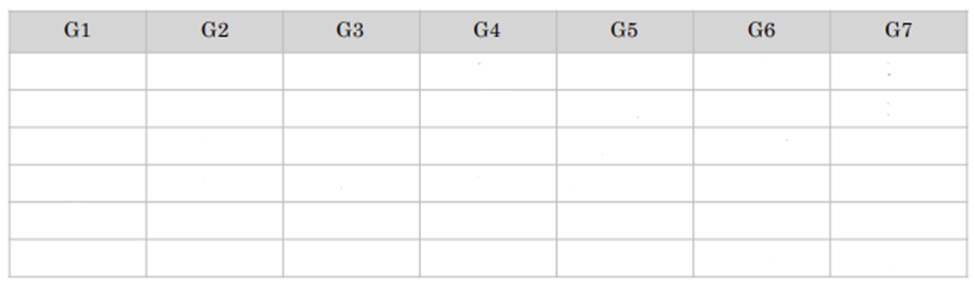
\includegraphics[width=0.8\textwidth]{assets/grid.png} % مسیر عکس را تغییر دهید
\end{center}
\bigskip
\bigskip
\rule{\linewidth}{0.4pt}

% Add more sections as needed...

\end{document}
